\subsection{Относительные гомологии и гомологически точная последовательность пары}

    Пусть $X$~--- топологическое пространство, $A \subset X$, тогда $\forall q \ C_{q}(A) \subset C_{q}(X)$ (вложение индуцирует мономорфизм цепей)
    и мы имеем морфизм цепных комплексов $(C_{\bullet}(X), \partial)$ и $(C_{\bullet}(A), \partial)$, то есть коммутативна следующая диаграмма:
    \begin{center}
        \includegraphics{lectures/0/pictures/cd_4}
    \end{center}
    Это так просто потому, что если у нас был симплекс $f\colon T^{q} \to A$, то его граница тоже целиком лежит в $A$,
    то есть $\partial f\colon T^{q - 1} \to A \in C_{q - 1}(A)$.

    Глядя на это, возникает естественная идея дополнить до короткой точной последовательности
    \[ 0 \to C_{q}(A) \to C_{q}(X) \to C_{q}(X)/C_{q}(A) \to 0 \]
    в каждом столбце.

    \begin{definition}
        Факторгруппу $C_{q}(X, A) \eqdef C_{q}(X)/C_{q}(A)$ называют \emph{относительными цепями}. 
    \end{definition}

    Построим цепной комплекс для относительных цепей, для этого надо определить дифференциалы.
    Это делается стандартно, возьмем $x \in C_{q}(A)$, тогда $\partial_{q}(x) \in C_{q - 1}(A)$, а значит
    композиция дифференциала и проекции пропустится через фактор:

    \begin{center}
        \includegraphics{lectures/0/pictures/cd_5}
    \end{center}

    Проверим теперь, что $\delta^2 = 0$. Действительно, из коммутаивной диаграммы выше мы понимаем, что
    \[ \delta_{q}(\overline{x}) = \delta_{q}(\pi_{q}(x)) = \pi_{q - 1}(\partial_{q}(x)) \Rightarrow \delta_{q - 1}(\delta_{q}(\overline{x})) = \delta_{q - 1}(\pi_{q - 1}(\partial_{q}(x))) = \pi_{q - 2}( \partial_{q - 1}(\partial_{q}(x))) = 0. \]

    Теперь мы построили цепной комплекс и можем определить относительные гомологии.
    \begin{definition}
        Пусть $X \subset A$, тогда относительными гомологиями мы будем называть гомологии комплекса относительных цепей, то есть
        \[ H_{q}(X, A) \eqdef \ker{\delta_{q}}/\Im{\delta_{q + 1}}. \]
    \end{definition}

    Теперь, попробуем получить для гомологий аппарат, идеологически похожий на теорему Зейферта-Ван-Кампена.

    Итак, мы имеем \emph{короткую точную последовательность комплексов}
    \[ 0 \to C_{\bullet}(A) \to C_{\bullet}(X) \to C_{\bullet}(X, A) \to 0\]
    В развёрнутом виде она представляет собой коммутативную диаграмму
    \begin{center}
        \includegraphics{lectures/0/pictures/cd_6}
    \end{center}
    в которой строки точны, а стлобцы~--- наши комплексы.

    \begin{theorem}[Точная последовательность пары]\label{LongExactSequenceOfPair}
        Существует \emph{связывающий гомоморфизм} $\varphi\colon H_{q}(X, A) \to H_{q - 1}(A)$, и соответственно, имеет место следующая длинная точная последовательность групп гомологий:
        \[ \ldots \to H_{q}(A) \to H_{q}(X) \to H_{q}(X, A) \xrightarrow{\varphi} H_{q - 1}(A) \to H_{q - 1}(X) \to \ldots \]
    \end{theorem}
    \begin{proof}
        На самом деле, это утверждение верно для любой точной последовательности комплексов. А именно, если
        последовательность цепных комплексов
        \[ 0 \to A_{\bullet} \to B_{\bullet} \to C_{\bullet} \to 0\]
        точна, то имеет место следующая длинная точность последовательность гомологий:
        \[ \ldots \to  H_{q}(A) \to H_{q}(B) \to H_{q}(C) \to H_{q - 1}(A) \to H_{q - 1}(B) \to \ldots\]

        Это можно без труда вывести из леммы о змее, проверив точность строк\footnote{\textcolor{magenta}{а так как это делается в абсолютно любом курсе гомологической алгебры, мне лень это сюда писать. }}
    \end{proof}

    \noindent\bf{Упражнение.}
    Докажите, что для $X \supset A \supset B$ имеет место следующая длинная точная последовательность групп гомологий
    \[ \ldots \to H_{q}(A, B) \to H_{q}(X, B) \to H_{q}(X, A) \to H_{q - 1}(A, B) \to \ldots \]

    Посмотрим, что всё это означает геометрически. Относительные циклы~--- это элементы
    \[ \Ker\lr*{C_{q}(X)/X_{q}(A) \to C_{q - 1}(X)/C_{q - 1}(A)}. \]
    Мы взяли представителя в $C_{q}(X)$, взяли границу и после факторизации по $C_{q - 1}(A)$ получили 0,
    а значит граница нашего цикла полностью лежит в $C_{q - 1}(A)$, то есть картинка имеет вид:
    \begin{center}
            \begin{tikzpicture}
            \node at (0,0){\includegraphics{lectures/0/pictures/pic_3}};
            \node at (-0.5, 0.5){\small \( A \)};
            \node at (3.2, 1.6){\small относительный цикл};
            \node at (-0.5, -1.8){\small абсолютный цикл \( \uparrow \)};
            \node at (1.8, 1.3){\small \( \swarrow \)};
            %	\draw[opacity=0.7] \foreach \x in {-4,...,5} {
	   (\x cm, 0.1) -- (\x cm, -0.1) node[below]{\tiny \x}
	   (\x cm - 0.5cm, 0.08) -- (\x cm - 0.5cm, -0.08)
	   \foreach \t in {1,2,3,4,6,7,8,9} {
	      (\x cm - 0.1 * \t cm, 0.055) -- (\x cm - 0.1 * \t cm, -0.055)
	   }
	};
	\draw[opacity=0.7,rotate=90] \foreach \x in {-3,-2,-1,1,2,3,4} {
	   (\x cm, 0.1) -- (\x cm, -0.1) node[right]{\tiny \x}
	   (\x cm - 0.5cm, 0.08) -- (\x cm - 0.5cm, -0.08)
	   \foreach \t in {1,2,3,4,6,7,8,9} {
	      (\x cm - 0.1 * \t cm, 0.055) -- (\x cm - 0.1 * \t cm, -0.055)
	   }
	};
;
            \end{tikzpicture}
    \end{center}
    С другой стороны, ясно, что $x \in C_{q}(X)/C_{q}(A)$~--- относительная граница, если $x + a = \partial(\ldots)$.

    \begin{remark}
        У связывающего гомоморфизма $H_{q}(X, A) \to H_{q - 1}(A)$ есть очень естественная интерпретация.

    Элементы $H_{q}(X, A)$~--- относительные циклы с точностью до относительных границ. Так как это оносительные $q$-мерные циклы,
    их граница лежит в  $A$, а значит, при взятии границы, мы получим как раз элемент $H_{q - 1}(A)$. То есть, связывающий гомоморфизм
    $H_{q}(X, A) \to H_{q - 1}(A)$~--- взятие границы.
    \end{remark}


    Рассмотрим также еще несколько важных следствий длинной точной последовательности пары. 

    \begin{corollary}\label{ParaCor1}
         Для любого топологического пространства $x$ и любой его точки $x_0 \in X$ мы имеем
        \[ H_{n}(X, x_0) = \widetilde{H}_{n}(X) \ \forall n. \]
    \end{corollary}
    \begin{proof}
        Запишем длинную точную последовательность приведенных гомологий пары $(X, x_0)$
        \[ \ldots \to  \widetilde{H}_{q}(x_0) \to \widetilde{H}_{q}(X) \to \widetilde{H}_{q}(X, x_0) \to \widetilde{H}_{q - 1}(x_0) \to \ldots \]
        Действительно, так как $\widetilde{H}_n(x_0) = 0 \ \forall n$, мы на самом деле имеем
        \[ \ldots \to 0 \to \widetilde{H}_{q}(X) \to \widetilde{H}_{q}(X, x_0) \to 0 \to \ldots, \]
        и из точности следует $\widetilde{H}_{q}(X) \cong \widetilde{H}_{q}(X, x_0) = H_{q}(X, x_0)$.
    \end{proof}

    \begin{corollary}
        Группы $H_{q}(X, A)$ измеряют различие между $H_{q}(X)$ и $H_{q}(A)$, а именно,
        \[ H_{q}(X, A) = 0  \quad \forall{q} \Rightarrow H_{q}(A) = H_{q}(X) \quad \forall q. \]
    \end{corollary}
    \begin{proof}
        Запишем длинную точную последовательность пары $(X, A):$
        \[ \ldots \to  H_{q}(A) \to H_{q}(X) \to H_{q}(X, A) \to H_{q - 1}(A) \to \ldots \]
        В нашем случае она имеет вид:
        \[ \ldots \to  H_{q}(A) \to H_{q}(X) \to H_{q}(X, A) \to H_{q - 1}(A) \to \ldots \]
        и из точности следует, что $H_{q}(A) \cong H_{q}(X)$.
    \end{proof}

    \noindent\bf{Упражнение.} Убедитесь, что верно и обратное утверждение.

    \subsection{Пары Боруска}

    \begin{definition}
        Пусть $X$ -- топологическое пространство, а $A \subset X$ с индуцированной топологией. Тогда говорят, что $(X, A)$ --
        \emph{пара Борсука} (или, \emph{корасслоение})\footnote{Еще говорят <<обладает свойством продолжения гомотопии>>, но это совсем уж длинно.}, если $\forall f \colon X \to Y, \ \forall F \colon A \times I \to Y$ такой, что $F|_{A \times 0} = f|_{A}$
        существует $G\colon X \times I \to Y$, причем такое, что $G|_{X \times 0} = f, \ G|_{A \times I } = F$.
    \end{definition}

    \begin{definition}
        Пара $(X, A)$ называется \emph{клеточной парой}, если $X$~--- клеточное пространство, $A$~--- клеточное подпространство $X$.
    \end{definition}

    \begin{remark}
       Так как очевидно, что $(D^n, \partial D^n)$~--- пара Борсука, клеточная пара является парой Борсука.
    \end{remark}   

    Нам от пар Борсука понадобится несколько базовых утверждений.


    \begin{theorem}[Характеризация пар Борсука]
        Если $(X, A)$~--- пара Борсука, то деформационная ретракция $X \times I$ на $X \cup (A \times I)$.
        Кроме того, если $A$~--- замкнуто, то верно и обратное.
    \end{theorem}
    \begin{proof}
    На картинке это выглядит следующим образом:
        \begin{center}
            \begin{tikzpicture}
            \node at (0,0){\includegraphics[scale = 0.7]{lectures/0/pictures/pic_4}};
            \node at (2.5, 1){\small \( A \times I \)};
            \node at (-1, -1){\small \( X \)};
            %	\draw[opacity=0.7] \foreach \x in {-4,...,5} {
	   (\x cm, 0.1) -- (\x cm, -0.1) node[below]{\tiny \x}
	   (\x cm - 0.5cm, 0.08) -- (\x cm - 0.5cm, -0.08)
	   \foreach \t in {1,2,3,4,6,7,8,9} {
	      (\x cm - 0.1 * \t cm, 0.055) -- (\x cm - 0.1 * \t cm, -0.055)
	   }
	};
	\draw[opacity=0.7,rotate=90] \foreach \x in {-3,-2,-1,1,2,3,4} {
	   (\x cm, 0.1) -- (\x cm, -0.1) node[right]{\tiny \x}
	   (\x cm - 0.5cm, 0.08) -- (\x cm - 0.5cm, -0.08)
	   \foreach \t in {1,2,3,4,6,7,8,9} {
	      (\x cm - 0.1 * \t cm, 0.055) -- (\x cm - 0.1 * \t cm, -0.055)
	   }
	};

            \end{tikzpicture}
        \end{center}

        Положим $Y = X \cup (A \times I)$, $f\colon X \to Y$~--- вложение. Рассмотрим теперь гомотопию $F_{t}(A) = A \times t$.
        Так как $(X, A)$~--- пара Борсука, существует $G\colon X \times I \to Y\colon G\vert_{A \times I} = F$.

        Докажем теперь в другую сторону:  пусть для $f\colon X \to Y$ есть гомотопия $F_{t}\colon A \to Y$, то
        есть отображение $F\colon X \cup (A \times I) \to Y$. Тогда искомое продолжение гомотопии~---
        композиция $F$ и деформационной ретракции $X \times I \to X \cup (A \times I)$\footnote{вот тут мы пользуемся замкнутостью $A$, так как нам нужно, чтоб покрытие было фундаментальным. }.
    \end{proof}

    \begin{corollary}
        Пара $(D^n, \Int(D^n))$~--- не пара Борсука. 
    \end{corollary}

    Вообще говоря, эта теорема показывает, что было бы хорошо, чтоб  $A$ было замкнутым.

    \begin{remark}
       В нехаусдорфовом случае бывает, что и с незамкнутым $A$ пара $(X, A)$ будет парой Борсука.
    \end{remark}

    \noindent\bf{Упражнение.} Если $(X, A)$~--- пара Борсука и $X$~--- Хаусдорфово, то $A$ замкнуто. 

    \begin{statement}\label{BorsukPairProp}
        Пусть $(X, A)$~--- пара Борсука. Тогда
        \[ X \cup CA \sim (X \cup CA)/CA = X / A.  \]
    \end{statement}
    \begin{proof}
        Рассмотрим вложение $X \to X \cup CA$. Прогомотопируем $A$ в вершину конуса $a$. Так как $(X, A)$~--- пара Борсука,
        эта гомотопия продолжается до гомотопии на $X$. Тогда финальный элемент гомотопии отображает $X \to X \cup CA$ так, что $A \mapsto a$,
        значит, это отображение пропускается через фактор $X/A$. С другой стороны ясно, как устроено обратное отображение $X \cup CA \to X/A$ (стягиваем конус в точку). Нетрудно заметить, что два построенных отображения задают гомотопическую эквивалентность.
    \end{proof}

    \begin{corollary}
         Если $(X, A)$~--- пара Боруска и $A$~--- стягиваемо, то $X \sim X/A$.
    \end{corollary}

    \begin{statement}
        Пара $(CX, X)$~--- всегда пара Борсука.
    \end{statement}

    \subsection{Относительные гомологии как абсолютные (факторизация)}

    Итак, в этом параграфе нас будет интересовать следующее (весьма полезное в вычислениях утверждение):

    \begin{theorem}
        В общем случае отображение $X \to X \cup CA$ индуцирует изоморфизм
        \[ H_{q}(X, A) \to H_{q}(X \cup CA, CA) = H_{q}(X \cup CA, a) = \widetilde{H}_{q}(X \cup CA), \]
        где $a$~--- вершина конуса.

        Если $(X, A)$~--- пара Борсука, то отображение проекции $p\colon X \to X/A, \ A \mapsto a$ индуцирует изоморфизм
        \[ H_{q}(X, A) \xrightarrow{p_{*}} H_{q}(X/A, a) = \widetilde{H}_{q}(X/A). \]
    \end{theorem}

    Вообще говоря, условие на $A$ во второй части теоремы часто опускают и говорят, что это верно для <<хороших пар>>. 
    Мы доказываем для пар Борсука, можно доказывать для случая, когда $A$~--- \emph{окрестностный деформационынй ретракт}.


    Для доказательства этой теоремы нам понадобится несколько важных (в общем контексте) лемм.

    Сначала посмотрим на геометрическую конструкцию \bf{барицентрического подразбиения}, чтоб
    иметь геометрическую интуицию в контексте сингулярных симплексов.

    Рассмотрим симплекс $[v_{0}, \ldots, v_{n}]$. его точки~--- линейные комбинации вида
     \[ \sum_{i = 0}^{n} t_i v_i, \quad \text{где} \sum_{i = 0}^{n} t_i = 1, \ t_i \ge 0. \]
    \begin{definition}
        \emph{Барицентр (центр тяжести)} симплекса~--- это точка $b \in [v_0, \ldots, v_n]$, у которой все барицентрические аоординаты $t_i$ равны, а именно,
        $t_i = \frac{1}{n + 1} \ \forall i$.

        \emph{Барицентрическое подразбиение (подразделение)} симплекса $[v_0, \ldots, v_n]$~--- это разбиение симплекса $[v_0, \ldots, v_n]$ на $n$-мерные симплексы
        $[b, w_0, \ldots, w{n - 1}]$, где по индукции $[w_0, \ldots, w_{n - 1}]$~--- $(n - 1)$-мерный симплекс барицентрического подразбиения грани $[v_0, \ldots, \hat{v}_i, \ldots, v_n]$.
        \begin{itemize}
            \item Индукция начинается с $n = 0$, когда барицентрическое подразбиение точки $[v_0]$ определяется просто, как сама точка $[v_0]$.
            \item В случае $n = 1$
        отрезок $[v_0 v_1]$ бьется на два отрезка $[v_0 b]$, $[b v_1]$, где $b$~--- середина отрезка $[v_0, v_1]$.
            \item В случае $n = 2$ треугольник $[v_0 v_1 v_2]$ бьется на 6 труегольников, образуемых его вершинами и точкой пересечения медиан $b$.
        \end{itemize}

        Из такого индуктивного определения следует, что вершины симплексов в барицентрическом подразбиении симплекса $[v_0 \ldots v_n]$~--- в точности барицентры всех
        $k$-мерных граней $[v_{i_0} \ldots v_{i_k}]$ симплекса $[v_0 \ldots v_n]$ для $0 \le k \le n$.

        При $k = 0$ это даёт нам просто набор вершин $v_i$. Барицентр симплекса $[v_{i_0} \ldots v_{i_k}]$ имеет барицентрические координаты
        $t_i = \frac{1}{k + 1}$ при $i = i_0, \ldots, i_k$ и $t_i = 0$ во всех остальных случаях.

    \end{definition}

    \begin{remark}
       Далее нам это не потребуется, но симплексы барицентрического подразбиения задают на симплексе $T$ структуру симплициального комплекса.
    \end{remark}









